\documentclass[a4paper]{article}

%% Language and font encodings
\usepackage[english]{babel}
\usepackage[utf8x]{inputenc}
\usepackage[T1]{fontenc}

%% Sets page size and margins
\usepackage[a4paper,top=3cm,bottom=2cm,left=3cm,right=3cm,marginparwidth=1.75cm]{geometry}

%% Useful packages
\usepackage{amsmath}
\usepackage{graphicx}
\usepackage[colorinlistoftodos]{todonotes}
\usepackage{hyperref}

\title{Book Bot Project}
\author{Group 7}

\begin{document}
\maketitle

\begin{abstract}
This file is a project report about Group 7's Book Bot Project for CmpE451 class. Information in this file is up to Milestone 1.
\end{abstract}

\section{Project Description}

 \qquad Book Bot Project is an assistant that can help users with everything related to books. It is a bot, and it works via Telegram. Working via Telegram makes the bot more accessible; users don't need to install anything extra and it is cross platform. \\
  
  
  \quad The base and most important functionality is to communicate with natural language. The bot can carry on a conversation with daily English. \\
 
  
  \quad Users can ask the bot about books. They can search books with different keywords, genres or authors, they can filter them in any way they want and they can sort them. They also can get information about specific books, see its current popularity via ratings or read the comments about the book.\\
 
  
  \quad Users can also give the bot feedback about the books they have read. They can comment on a book or rate a book. This will help the bot learn more about what the user likes and help it work more user oriented \\
 
  
  \quad The bot can also recommend the user some books depending on their previous ratings and taste of books.

\subsection{Project Requirements}

We have defined our project requirements as follows and our customer has agreed and approved the requirements. Note that the following is a summary of the detailed requirements page. You can see the full list from \href{https://github.com/bounswe/bounswe2017group7/wiki/Project-Requirements}{project requirements} in our wiki page.

\begin{enumerate}
\item Functional Requirements
  \begin{enumerate}
  \item System Requirements
    \begin{enumerate}
    \item Telegram will be the medium for the bot.
    \item Goodreads or Google Books will be our source of book related information.
    \item Wit.ai will be used for NLP purposes to understand natural language.
    \item There will be regular users, admins and moderators.
    \item There will be a conversation tree which is going to be used to determine the conversation direction.
    \end{enumerate}
  \item User Requirements
    \begin{enumerate}
    \item We will have regular users as Telegram Users.
    	\begin{enumerate}
        \item Users will be able to get information; search for books, filter them, sort them and read comments about them
        \item Users will be able to give feedback about books; comment on them and rate them.
        \item Users will be able to get book recommendations.
        \end{enumerate}
    \item We will have admin users.
        \begin{enumerate}
        \item Admins will be able to modify the conversation tree
        \item Admins will be able to see and flag comments
        \item Admins will be able to see and block users
        \end{enumerate}
    \item We will have moderator users.
        \begin{enumerate}
        \item Moderators will be able to see and flag comments
        \item Moderators will be able to see and block users
        \end{enumerate}
    \end{enumerate}
  \end{enumerate}
\item Non Functional Requirements
  \begin{enumerate}
  \item Speed: We are creating a bot which users can chat with so the response time cannot be more than 5 seconds.
  \item Size: We want our bot to be portable an not bulky, we will use the Telegram as our medium hence the user won't need extra space for the bot.
  \item Usage: It should be easy to use, there shouldn't be any training time.
  \item Requirements: Bot needs internet connection to work.
  \item Failures: If bot fails, it shouldn't take more than ten minutes to restart the system and get it working again.
  \item Target devices: We are targeting all platforms in which Telegram works.
  \item User Satisfaction: Bot should keep track of the success of its recommendations by tracking the ratings of the recommended books.
  \end{enumerate}
\end{enumerate}
\newpage

\subsection{Project Design}

See \autoref{fig:design}

\begin{figure}[!hb]
  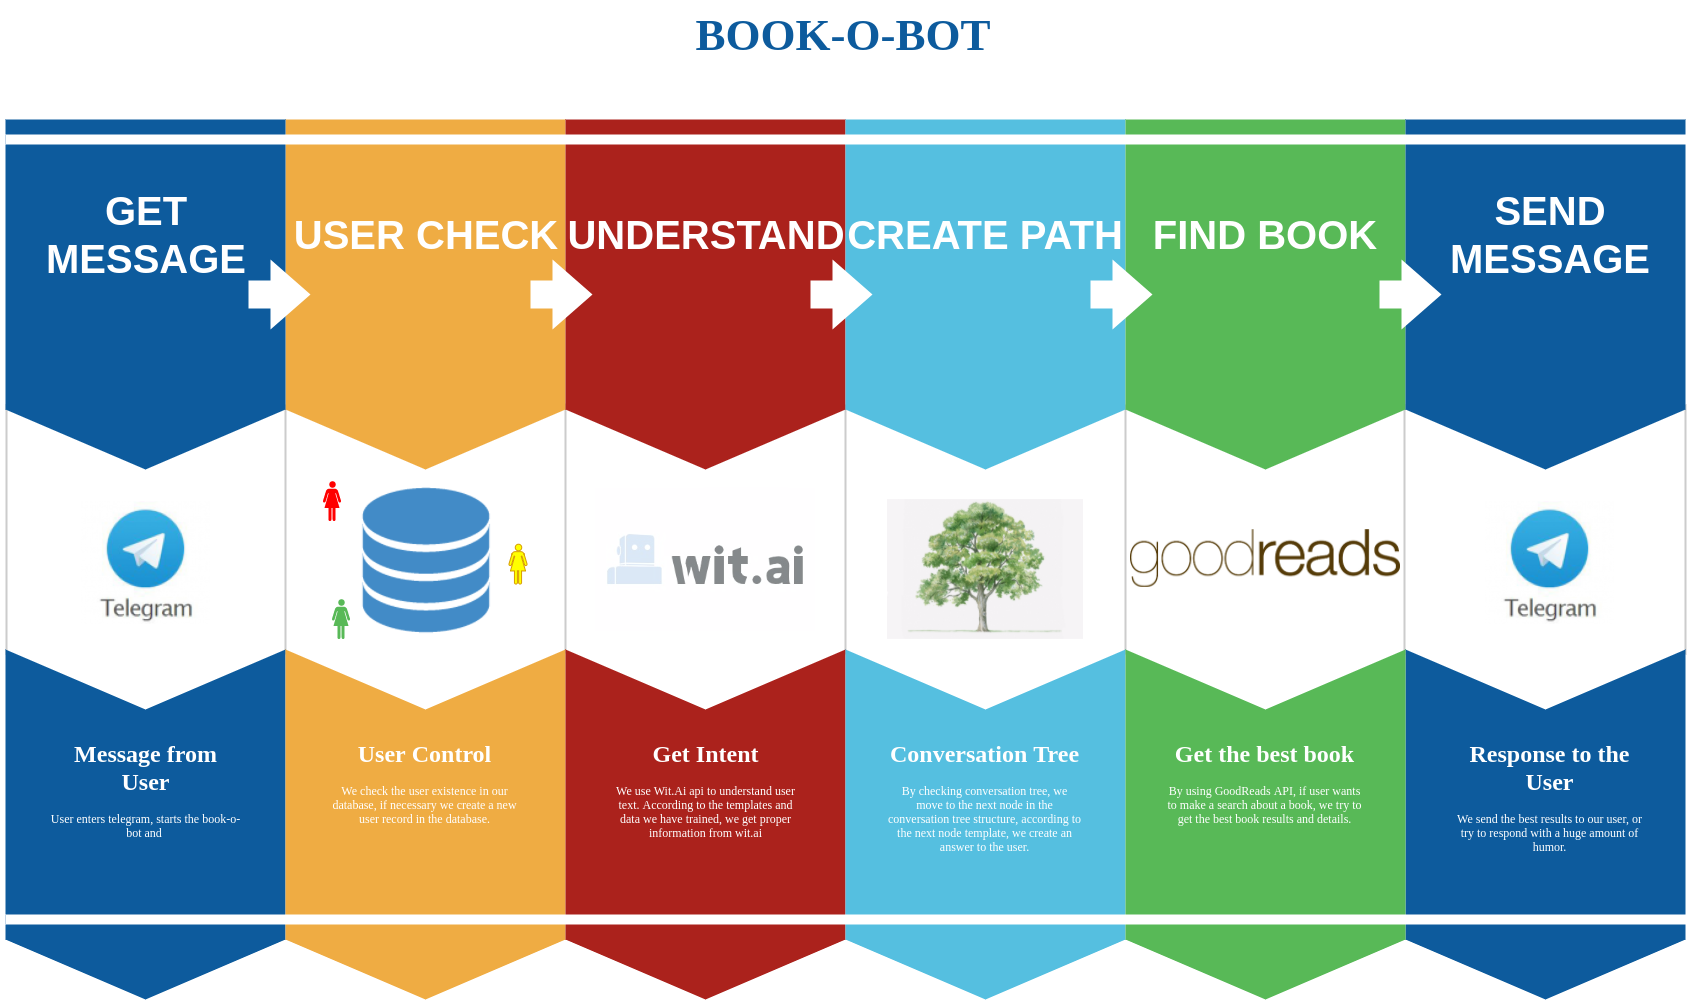
\includegraphics[width=\linewidth]{figures/design.png}
  \caption{Project Design}
  \label{fig:design}
\end{figure}


\newpage

\subsection{Project plan}

TODO: write project plan. It is going to be in tabular form. See Table~\ref{tab:projectplan}

\begin{table}
\centering
\begin{tabular}{l|r}
Row Name & Row Name \\\hline
Column Name & column value \\
Column Name & column value
\end{tabular}
\caption{\label{tab:projectplan}An project plan table.}
\end{table}

\section{Project Milestones}
\subsection{Milestone 1}
TODO: Milestone 1
\subsection{Milestone 2}
TODO: Milestone 2
\subsection{Final Milestone}
TODO: Final Milestone

\section{Project status}
\subsection{Deliverable List}

\begin{enumerate}
\item One
  \begin{enumerate}
  \item One point one: Explanation
  \item One point to: What is this deliverable
  \end{enumerate}
\item Two.
\end{enumerate}

\subsection{Deliverable Status}
TODO: write deliverable status. It is going to be in tabular form. See Table~\ref{tab:deliverablestatus}

\begin{table}
\centering
\begin{tabular}{l|r}
Row Name & Row Name \\\hline
Column Name & column value \\
Column Name & column value
\end{tabular}
\caption{\label{tab:deliverablestatus}An deliverable status table.}
\end{table}

\subsection{Deliverable Evaluation}
TODO: Evaluate

\newpage
\section{Coding Work}
You can find each team member's contribution to the code in the ~\autoref{tab:codingwork}

\begin{table}[!hb]
\centering
\begin{tabular}{l|r}
Name & Coding Work \\\hline
Salih Sevgican & GoodReads API implementation \\ 
 & book API class for ease of use \\
 & Main Page of the project (Front End)\\
 & AWS has been configured for the deployment\\
 & Updated requirements.txt\\
 & GoodReads compatibility with TelegramBot tested on telegramapi\\\hline
Irmak Kavasoglu & Initial environment setup for Django \\
& Setting up database model for Telegram User \\
& Setting up database model for Templates \\
& Setting up database model for Conversation Node \\
& Integrating Mptt tool for conversation tree \\
& Registering models to admin page and customizing their look \\\hline
Add your name & add your contribution
\end{tabular}
\caption{\label{tab:codingwork}Coding work table.}
\end{table}

\section{Evaluation of tools and managing the project}
\subsection{Django}
\subsection{Mptt}
\subsection{Telegram}
\subsection{Wit}
\subsection{GoodReads}

\quad GoodReads API is very useful to make a search about a book by given any kind of keyword. Keyword can be related to author, genre or title, doesn't matter, this api makes a succesfull search every time. We've used a wrapper library for GoodReads API which made easy to write methods for search types. Library is a litlle bit complicated despite it is written to ease our job. Unfortunately not every book is being hold as a same type in goodreads database, some of queries returns arrays with additional information of book such as order number of a book in the book series, and some of queries returns just the name of book. This is an issue we need to handle very well in order to make a great impression with the responds to the bot user.  
\subsection{AWS}

\section{Summary}
TODO fill

\end{document}